%&"../main"
\documentclass[../main]{subfiles}
\begin{document}

\chapter{电磁波的极化}%
\label{cha:电磁波的极化}

\section{实验目的}%
\label{sec:\arabic{chapter}实验目的}

研究线极化、圆极化和椭圆极化电磁波的产生和各自的特点。

\section{实验内容}%
\label{sec:\arabic{chapter}实验内容}

\begin{enumerate}

	\item 圆极化波的调整与测试;

	\item 线极化波的调整与测试;

	\item 椭圆极化波的调整与测试。

\end{enumerate}

\section{实验原理与说明}%
\label{sec:\arabic{chapter}实验原理与说明}

\subsection{所使用的实验仪器}%
\label{sub:\arabic{chapter}所使用的实验仪器}

\begin{table}[htbp]
	\centering
	\caption{实验仪器}
	\label{tab:\arabic{chapter}实验仪器}
	\csvautobooktabular{tab/1/BOM.csv}
\end{table}

实验系统框图如图\ref{fig:实验系统框图}所示。

\begin{figure}[htbp]
	\centering
	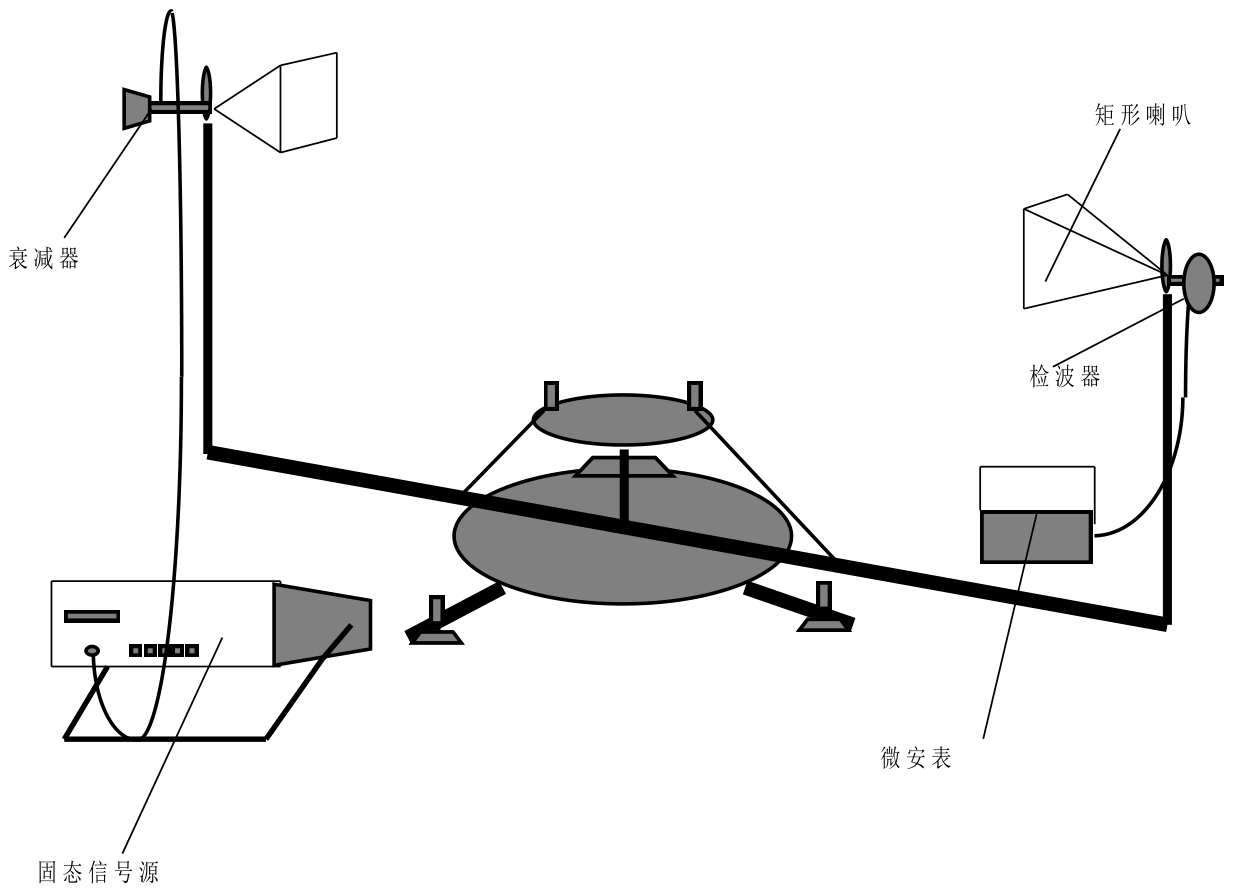
\includegraphics[width = 0.8\linewidth]{2/instruction.png}
	\caption{实验系统框图}
	\label{fig:实验系统框图}
\end{figure}

电磁波综合测试仪中辐射喇叭(\SI{3}{\cm}波段)支路由固态信号源、频率计(或波长计
) 、衰减器及圆形喇叭等组成。固态信号源的工作频率$ f = \SI{9370}{\MHz} $左右,接
收喇叭支路由矩形喇叭、检波器、微安表等组成。

\subsection{原理}%
\label{sub:\arabic{chapter}原理}

电磁波极化是指电磁波在无限大均匀媒质中传播时,空间某点上电场强度矢量$ \bm{E} $的
末端随时间变化的轨迹。当电场矢量末端总在一直线上周期地变化时,称为线极化波;当电
场矢量末端轨迹是圆或椭圆时,即电场矢量末端总在圆或椭圆上周期地变化时,称为圆极化
波或椭圆极化波。无论是线极化波,左、右旋圆极化波,左、右旋椭圆极化波,都可由两个
同频率且场矢量相互正交的线极化波组合而成。本实验利用方圆波导转换,介质圆波导和圆
锥喇叭连接而成的电磁波极化天线,分别研究波的极化——线极化波、圆极化波和椭圆极化波
的特性。

\begin{figure}[htbp]
	\centering
	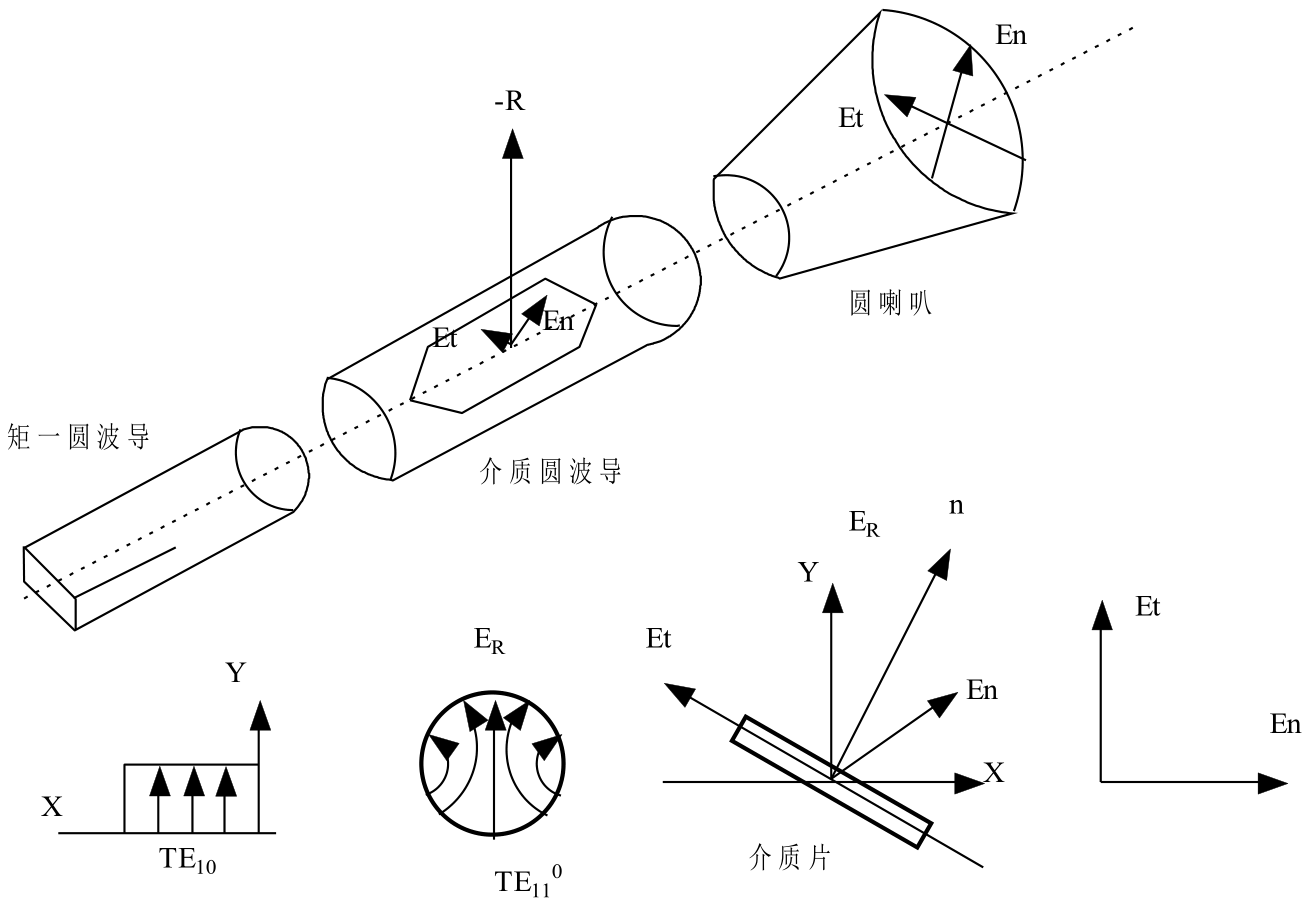
\includegraphics[width = 0.8\linewidth]{2/device.png}
	\caption{圆极化波辐射装置}
	\label{fig:圆极化波辐射装置}
\end{figure}

图\ref{fig:圆极化波辐射装置}所示为圆极化波辐射装置,其中介质圆波导可做
\ang{360;;}旋转,并有刻度指示转动的角度。当TE波经方圆波导转换到圆波导口面时则过
渡为TE波,并在介质圆波导内分成两个分量的波,即垂直界面片平面的一个分量和平行介质
面的一个分量。实验装置设计为\SI{9370}{\MHz}左右使两个分量的波相位差\ang{90;;},
适当调整介质圆波导(亦可转动介质片)的角度使两个分量的幅度相等时则可得到圆极化波
。当方圆波导使$ \mathrm{TE}_{10} $的EY波过渡到$ \mathrm{TE}_{11} $成为RP波后,在
装有介质片的圆波导段内分成$ E_\mathrm{t} $和$ E_\mathrm{n} $两个分量的波,因$ E_\mathrm{t} $
和$ E_\mathrm{n} $的速度不同,$ v_\mathrm{c} = v_\mathrm{n} > v_\mathrm{t} =
\dfrac{v_\mathrm{c}}{\sqrt{\varepsilon_\mathrm{r}}} $ 当介质片的长度$ L $ 取得合
适时,使$ E_\mathrm{n} $波的相位超前 $ E_\mathrm{t} $ 波的相位 \ang{90;;},这就
实现了圆极化波相位条件的要求;为使$ E_\mathrm{t} $和 $ E_\mathrm{n} $的幅度相等
,可使介质片的$ n $方向跟 $ y $轴之间夹角为\ang{45;;},若介质片的损耗略去不计,
则有,实现了圆极化波幅度条件的要求(有时需稍偏离 \ang{45;;} 以以实现幅度相位的要
求)。为了确定圆极化波右旋、左旋的特性,把$ n $转到$ y $方向符合右手螺旋规则的波
,定为右旋圆极化波;把$ n $转到$ y $方向符合左手螺旋规则的波,定为左旋圆极化波。
波极化天线除作为圆极化波工作外,也可作线极化波,椭圆极化波工作使用。当作线极化波
工作时,介质片$ n $与$ y $轴相垂直(或平行)。当作椭圆极化波工作时,介质片$ n $
与$ y $夹角可在$ \alpha = \ang{0;;} - \ang{45;;} $之间。

\section{实验步骤}%
\label{sec:\arabic{chapter}实验步骤}

\subsection{圆极化波的调整与测试}%
\label{sub:圆极化波的调整与测试}

根据圆极化波的条件,两个同频率的正交场相干波必须幅度相等,相位差$ \pm \dfrac{\pi
}{2} $ 为此将反射板和介质板拿掉,把辐射喇叭换成圆喇叭,转动圆喇叭使介质片的$ n $
方向跟$ y $轴之间夹角为\ang{45;;}左右,然后固定圆喇叭,再把接收喇叭调整到与圆喇
叭成一直线。转动接收喇叭,每隔\ang{10;;}测量一次,读取微安表上的读数,并填入表
\ref{tab:圆极化波调整与测试数据表} ,最后算出圆极化波的椭圆度$ e =
\sqrt{\dfrac{I_\mathrm{min}}{I_\mathrm{max}}} $ 值为0.7651。

\begin{table}[htbp]
	\centering
	\caption{圆极化波调整与测试数据表}
	\label{tab:圆极化波调整与测试数据表}
	\csvautobooktabular{tab/2/circle.csv}
\end{table}

\subsection{线极化波的调整与测试}%
\label{sub:线极化波的调整与测试}

转动圆喇叭使介质片的$ n $方向跟$ y $轴之间夹角为\ang{0;;}或\ang{90;;},就可以得
到线极化波。固定圆喇叭,转动接收喇叭,每隔\ang{10;;}测量一次,读取微安表上的读数
,并填入表\ref{tab:线极化波的调整与测试数据表}。

\begin{table}[htbp]
	\centering
	\caption{线极化波的调整与测试数据表}
	\label{tab:线极化波的调整与测试数据表}
	\csvautobooktabular{tab/2/line.csv}
\end{table}

\subsection{椭圆极化波的调整与测试}%
\label{sub:椭圆极化波的调整与测试}

调整与测试椭圆极化波的方法与内容同章节\ref{sub:圆极化波的调整与测试}和
\ref{sub:线极化波的调整与测试},要注意的是圆喇叭的转角在\ang{0;;},\ang{45;;} 之
间,按表\ref{tab:椭圆极化波的调整与测试数据表}列出记录表格,最后计算出椭圆极化波
的椭圆度$ e = \sqrt{\dfrac{I_\mathrm{min}}{I_\mathrm{max}}} $ 值为0.6009。

\begin{table}[htbp]
	\centering
	\caption{椭圆极化波的调整与测试数据表}
	\label{tab:椭圆极化波的调整与测试数据表}
	\csvautobooktabular{tab/2/oval.csv}
\end{table}

\section{实验结果}%
\label{sec:\arabic{chapter}实验结果}

实验数据见表\ref{tab:圆极化波调整与测试数据表},
\ref{tab:线极化波的调整与测试数据表}和\ref{tab:椭圆极化波的调整与测试数据表}。

\section{讨论}%
\label{sec:\arabic{chapter}讨论}

这次实验比上一个简单。但注意到电流表示数抖动得非常剧烈。要过很长时间才能停下来。
如果在还不稳定的时候读数,数据会很不准确。

\section{结论}%
\label{sec:\arabic{chapter}结论}

实验中遇到的问题依旧来自于实验仪器,学长调试之后发现方喇叭必须稍微倾斜一个小角度
才行。而正常的仪器都是水平的。

\section{思考题}%
\label{sec:\arabic{chapter}思考题}

\begin{Exercise}

	一右旋圆极化波从空气正入射到另一种媒质表面,反射波与透射波的旋向如何(左
	旋还是右旋)?

\end{Exercise}

\begin{Answer}

	因为介质的折射率都大于空气,垂直极化波的反射波有半波损失,也即相位滞后
	\ang{180;;}。而平行极化波的反射波没有半波损失。所以如果原来是右旋圆极化
	,垂直极化分量超前\ang{90;;},那么反射之后垂直极化分量就滞后\ang{90;;},
	成为左旋圆极化波。而透射波没有半波损失。反射波的旋向为左旋,透射波的旋向
	为右旋。

\end{Answer}

\end{document}

